\documentclass[../main.tex]{subfiles}
 
\begin{document}

\subsection{ H.264 Profiles}

H.264 specification includes several profiles, each specifying a subset of the optional features in the H.264 standard. A Profile places limits on the algorithmic capabilities
required of an H.264 decoder. Each Profile is intended to be useful to a class of
applications. For example, the Baseline Profile may be useful for low-delay, such as video conferencing, with relatively low computational requirements. The
Main Profile may be suitable for basic television/entertainment applications such as Standard
Definition TV services. The High Profiles add tools to the Main Profile which can improve compression efficiency especially for higher spatial resolution services, such as High Definition TV.



\subsection{ Main Decoding Processes }

The decoding process is carried out by an H.264 video decoder. Flow diagram is shown in Figure \ref{fig:decproc}.

\begin{figure} [ht]
\begin{center}
\begin{tabular}{c} %% tabular useful for creating an array of images 
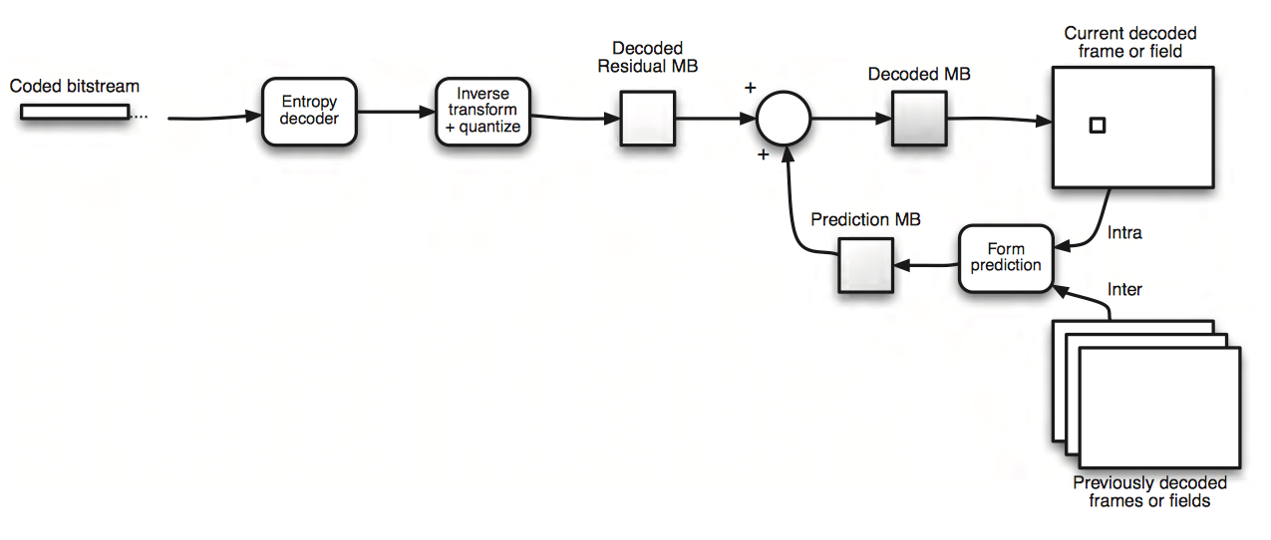
\includegraphics[height=5cm]{dec_proc.png}
\end{tabular}
\end{center}
\caption[decproc] 
{ \label{fig:decproc} H.264 decoding process \cite{richardson2004h} }
\end{figure} 

Initially, decoder codes compressed bitstream and does entropy decoding, obtaining a coefficient matrix. The following steps are dequantization and IDCT. Residual is output of this stage. Then the decoder will decode the frame depending on the combination of residual and prediction results. Notice that, in the both of coder and decoder, data is processed in units of macroblock. A decoded residual macroblock is formed by re-scaling and inverse transformation. Prediction is created in decoder and is added to the residual to generated a decoded macroblock. 

\subsubsection{ Parsing Process with Entropy Decoding }

As shown in Figure \ref{fig:parsing}, inputs to parsing process are bitstream from contents of video slices. Output of this process are syntax element values. (Video sequence that is represented in a particular format which is syntax).

\begin{figure} [ht]
\begin{center}
\begin{tabular}{c} %% tabular useful for creating an array of images 
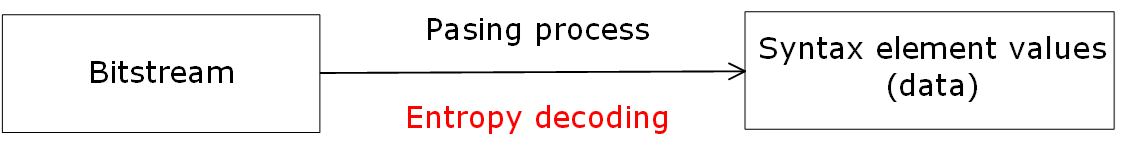
\includegraphics[width=0.5\textwidth]{parsing.png}
\end{tabular}
\end{center}
\caption[parsing] 
{ \label{fig:parsing} Entropy decoding process}
\end{figure} 

Actually, several methods are specified by H.264 for coding symbols, including Fixed Length Code, Exponential-Golomb variable length code, CAVLC and CABAC. 

And the data can be divided into two parts: decoder controlling parameters and transform coefficients. Above the slice data level, bits are decoded using Fixed Length decoder or Exp-Golomb decoder. In the slice data level and below, coefficient values are decoded in one of two ways. In CABAC mode, all symbols are decoded by CABAC decoder. Otherwise, coefficient values using CAVLC and other symbols are coded using fixed length or Exp-Golomb decoder. In our baseline decoder, Exp-Golomb and CAVLC are utilized.

\subsubsection{ Exponential Golomb Decoder }

Exponential Golomb codes (ExpG) are an efficient way of representing data symbols with varying probabilities. It assigns short codewords to frequently-occurring data symbols and long codewords to less common data symbols. A parameter $code\_num$ indicates codewords. The length of Exponential-Golomb codes are varying with two properties:

\begin{enumerate}
\item With the increase of $code\_num$, code length also rises.
\item Without looking up for tables, each code can be generated and decode algorithmically. 
\end{enumerate}

The structure of an Exp-Golomb codeword:

\[ [\text{Zero prefix}]\ 1\ [\text{Information}] \]

The codeword consists of $M$ zero prefix ($M \geq 0$, $M$ is an integer), a one and $M$-bit information. The length of the codeword is $2M+1$ bit.

The process of decoding $code\_num$ is followed: 

\begin{enumerate}
\item The decoder reads $M$ consecutive zeros and calculates the total length of the next Exp-Golomb codeword as $2M + 1$ bits. 
\item Read a one and ignore it.
\item It reads the remaining $M$ bits and calculates $code\_num$ which is then mapped to $k$ (data).
\end{enumerate}

There is an example:

\[ codeword = \underbrace{0000000}_\text{Zero Prefix} \textbf{1} \underbrace{1100011}_\text{Info.}  \]

% \begin{figure} [ht]
% \begin{center}
% \begin{tabular}{c} %% tabular useful for creating an array of images 
% 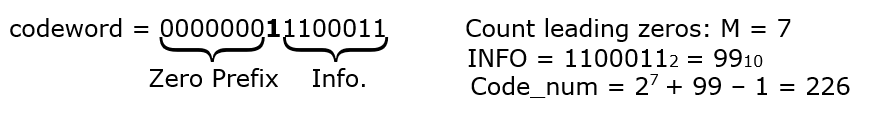
\includegraphics[width=0.5\textwidth]{expG.png}
% \end{tabular}
% \end{center}
% \caption[expG] 
% { \label{fig:expG} Exp-Golomb decoding process}
% \end{figure} 

The codeword to be decoded has 7 leading zeros and a one, followed by the information code $1100011$ which will be converted to decimal number. Then we calculate the result $code\_num$ depending on the formula: 

\[ code\_num = 2M + \text{Information} - 1 \]

Then $code\_num$ is mapped to $k$ (data) according to different mapping types which is shown in Table \ref{tab:mapping}.

% \begin{figure} [ht]
% \begin{center}
% \begin{tabular}{c} %% tabular useful for creating an array of images 
% 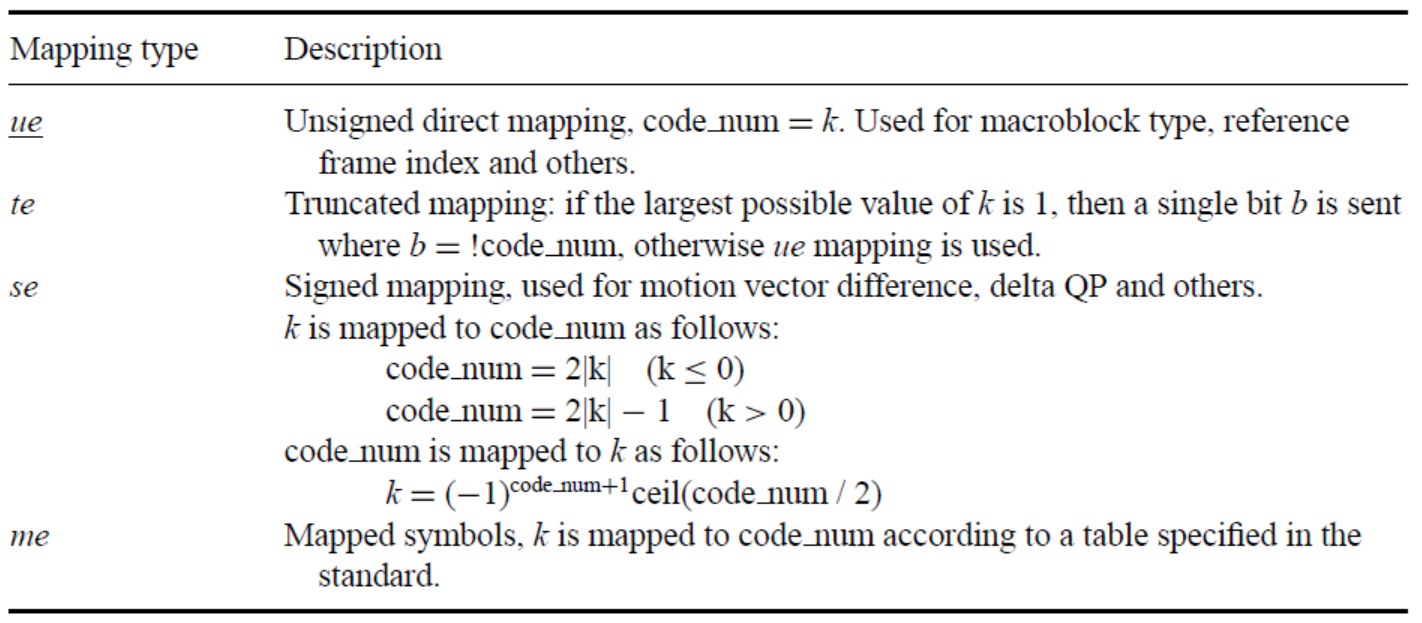
\includegraphics[width=0.8\textwidth]{mapping.png}
% \end{tabular}
% \end{center}
% \caption[mapping] 
% { \label{fig:mapping} Code number mapping methods}
% \end{figure} 

\begin{table}[ht]
% \label{tab:mapping}
\begin{center}       
\begin{tabular}{|l|p{10cm}|} 
\hline
\rule[-1ex]{0pt}{3.5ex} Mapping type & Description \\  
\hline
\rule[-1ex]{0pt}{3.5ex} $ue$ & Unsigned direct mapping.
\[code\_num = k\]
Used for macroblock type, reference frame index and others. \\  
\hline
\rule[-1ex]{0pt}{3.5ex} $te$ & Truncated mapping: if the largest possible value of $k$ is 1, then a single bit $b$ is sent where $b = !code\_num$, otherwise $ue$ mapping is used. \\
\hline
\rule[-1ex]{0pt}{3.5ex} $se$ & Signed mapping, used for motion vector difference, delta QP and others. $k$ is mapped to $code\_num$ as follows: 
\[code num = 2|k| \quad (k \leq 0) \] 
\[code num = 2|k| - 1 \quad (k > 0) \] 

$code\_num$ is mapped to $k$ as follows:
\[k = (−1)^{code\_num + 1}ceil(code\_num / 2) \] \\
\hline
\rule[-1ex]{0pt}{3.5ex} $me$ & Mapped symbols, $k$ is mapped to $code\_num$ according to a table specified in the standard. \\
\hline
\end{tabular}
\end{center}
\caption[mapping]{\label{tab:mapping} Code number mapping types\cite{richardson2004h} } 
\end{table}

\subsubsection{ Context Adaptive Variable Length Coding (CAVLC) }
Residual, the transform coefficients are decoded by CAVLC decoder. Each $8 \times 8$ block of quantized transform coefficients is processed as four $4 \times 4$ blocks for the purposes of CAVLC encoding and decoding. The decoding process can be divided into 5 stages:

    1. Decode the number of coefficients and trailing ones
    
    2. Decode the sign of each trailing ones
    
    3. Decode the levels of the remaining non-zero coefficients
    
    4. Decode the number of zeros preceding each non-zero coefficient
    
    5. Zero padding 

Decode the number of coefficients and trailing ones, according to input bitstream and standard table 9-5. Then the result is used to decode sign of trailing ones. To decode the levels of the remaining coefficients, we need to obtain the suffix length and get level prefix depending on standard table 9-6. The next step is to decode the number of zeros preceding each non-zero coefficient. The total number of coefficients and standard table 9-7 are needed. After the four steps, use zero to pad the remaining elements.

\subsection{Prediction Overview}

The prediction methods may have a great influence on the compression performance.H.264 supports two prediction options: \textbf{Intra prediction} using data within
the current frame, \textbf{Inter prediction} using motion compensated prediction from previously
coded frames. H.264 provides multiple prediction block sizes, multiple reference frames and special modes. All these features give H.264 a great deal of flexibility in the prediction process. By selecting the best prediction options for an individual macroblock, H.264 can minimize the residual size to produce a highly compressed bitstream.



\subsubsection{ Macroblocks In Prediction }

H.264 divides each frame in the video into “macroblocks,” which are blocks of 16x16
pixels. The macroblocks are decoded from left to right, and then top to bottom. There are three types of marcoblocks for prediction sources, an I Macroblock, a P Macroblock and a B Macroblock. An I Macroblock (I MB) is predicted using intra prediction from
neighboring samples in the current frame. A P Macroblock (P MB) is predicted from samples
in a previously-coded frame which may be before or after the current picture in display order.  Each partition in a B Macroblock (B MB) is
predicted from samples in one or two previously-coded frames. (Figure \ref{fig:mbtypes})

  \begin{figure} [ht]
   \begin{center}
   \begin{tabular}{c} %% tabular useful for creating an array of images 
   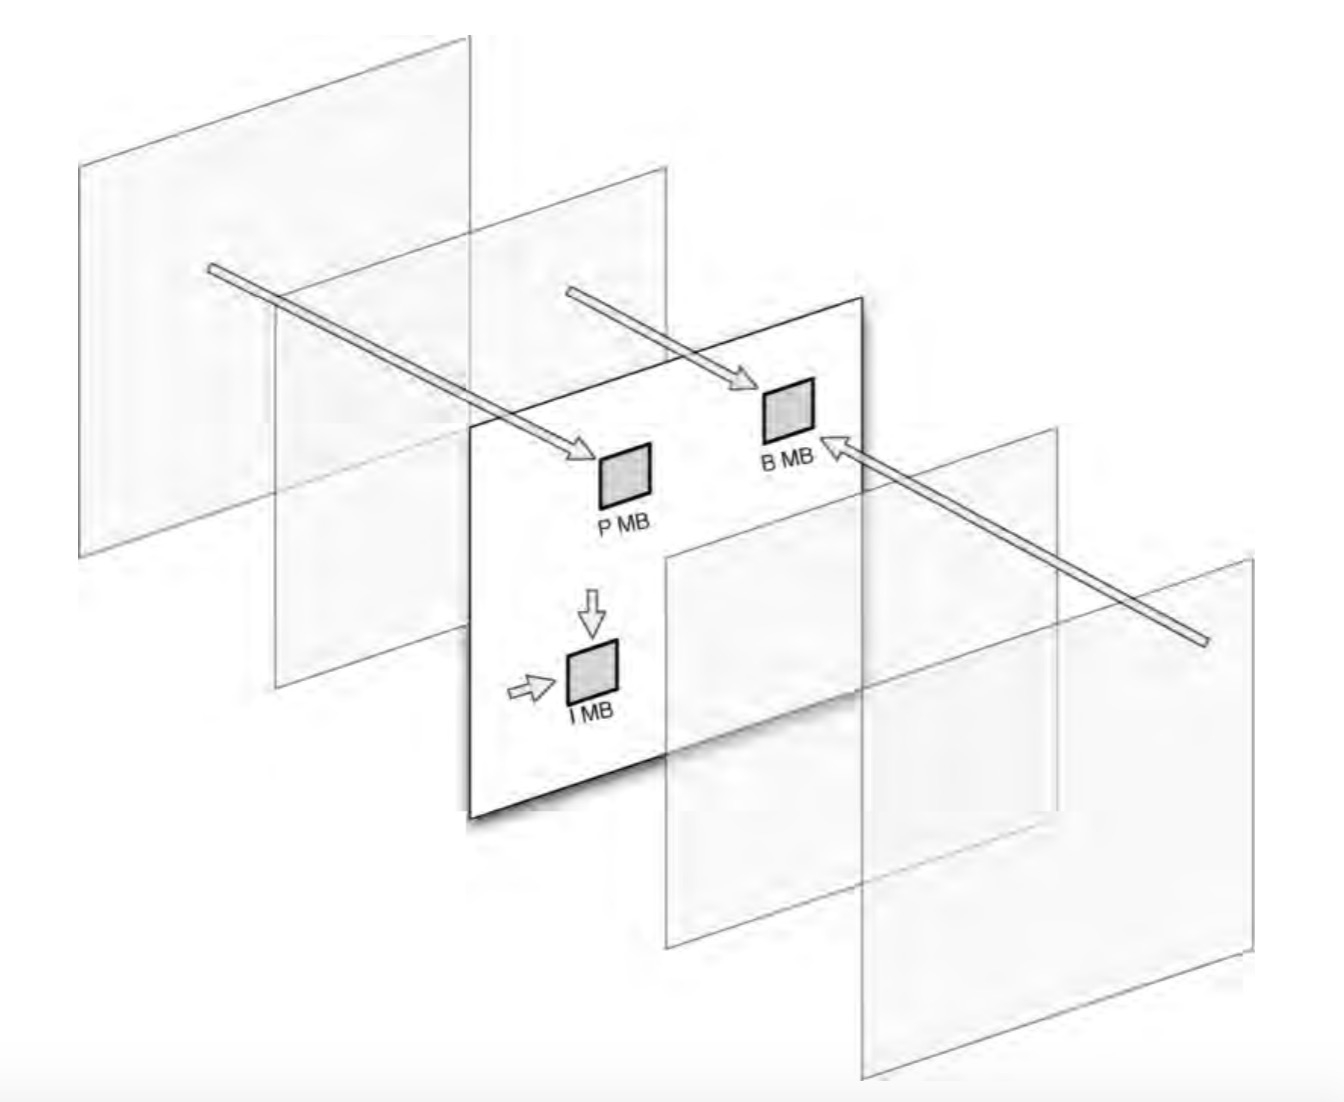
\includegraphics[height=5cm]{marcoblock.jpg}
   \end{tabular}
   \end{center}
   \caption[mbtypes] 
%>>>> use \label inside caption to get Fig. number with \ref{}
   { \label{fig:mbtypes} Marcoblock types \cite{richardson2004h} }
   \end{figure}     % 在reference中引用

\subsubsection{ Intra-Prediction }

Intra prediction is used to use part of the frame
to predict the other parts. An I Macroblock (I MB) is predicted using intra prediction from neighbouring samples in the current frame. For every block of the frame up to 16x16 pixels, intra-prediction uses previously decoded neighbor blocks to give an estimate for the new
block. 

In an intra macroblock, there are three choices of intra prediction block size for the luma
component, namely $16 \times 16$, $8 \times 8$ or $4 \times 4$. A single prediction block is generated for each
chroma component. Each prediction block is generated using one of a number of possible
prediction modes.(Figure \ref{tab:predtypes}) 

\begin{table}[ht]
\label{tab:predtypes}
\begin{center}       
\begin{tabular}{|l|p{10cm}|} 
\hline
\rule[-1ex]{0pt}{3.5ex}  Intra prediction block size & Notes\\  
\hline
\rule[-1ex]{0pt}{3.5ex}  $16 \times 16$ (luma) &  A single $16 \times 16$ prediction block P is generated.   \\
\hline
\rule[-1ex]{0pt}{3.5ex}  $8 \times 8$ (luma) & An $8 \times 8$ prediction block P is generated for each $8 \times 8$ luma block.
 \\
\hline
\rule[-1ex]{0pt}{3.5ex}  $4 \times 4$ (luma) & A $4 \times 4$ prediction block P is generated for each $4 \times 4$ luma block.   \\
\hline
\rule[-1ex]{0pt}{3.5ex}  Chroma & One prediction block P is generated for each chroma component.
Four possible prediction modes. The same prediction mode is used
for both chroma components.  \\
\hline

\end{tabular}
\end{center}
\caption{Intra prediction types\cite{richardson2004h} } 
\end{table}

$4 \times 4$ luma has 9 prediction modes, which are shown in Figure \ref{fig:4x4predmodes}. The samples, labeled A-M, have previously been decoded and reconstructed and they act as the prediction reference, then decoder copies the reference samples to the currently decoding blocks to continue the decode process.
and decoder to form a prediction reference. 

 \begin{figure} [ht]
   \begin{center}
   \begin{tabular}{c} %% tabular useful for creating an array of images 
   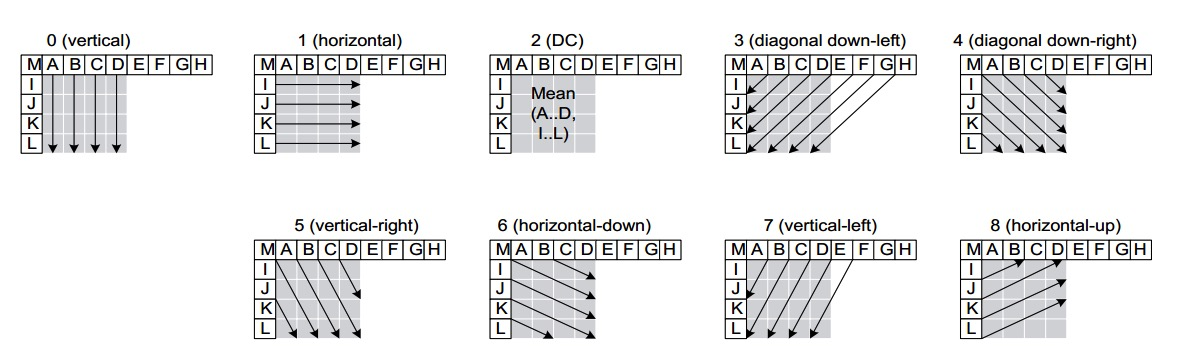
\includegraphics[height=5cm]{44intraprediction.jpg}
   \end{tabular}
   \end{center}
   \caption[predmodes] 
%>>>> use \label inside caption to get Fig. number with \ref{}
   { \label{fig:4x4predmodes} 
$4 \times 4$ intra prediction modes \cite{richardson2004h} }
   \end{figure}     % 在reference中引用
   
As an alternative to the $4 \times 4$ luma modes, the entire $16 \times 16$ luma component
of a macroblock may be predicted in one operation. Four modes are available.(Figure \ref{fig:16x16predmodes})
%此处文字应该在上下两图中间

\begin{figure} [ht]
   \begin{center}
   \begin{tabular}{c} %% tabular useful for creating an array of images 
   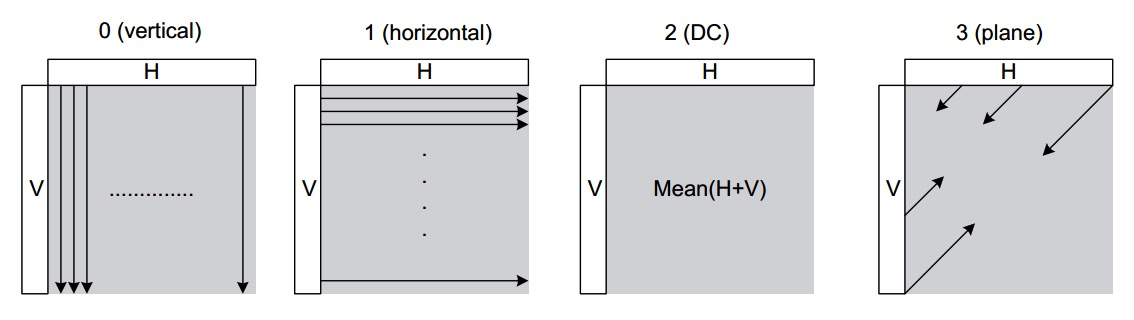
\includegraphics[height=5cm]{1616intraprediction.jpg}
   \end{tabular}
   \end{center}
   \caption[16x16predmodes] 
%>>>> use \label inside caption to get Fig. number with \ref{}
   { \label{fig:16x16predmodes} 
$16 \times 16$ intra prediction modes \cite{richardson2004h} }
   \end{figure}     % 在reference中引用
   
Intra prediction of the luma component with an $8 \times 8$ block size is only available in the High
profiles. Each $8 \times 8$ luma block in a macroblock is predicted using one of nine
prediction modes which are as same as the nine modes of $4 \times 4$ luma.
   
Each chroma component of a macroblock is predicted from previously encoded chroma
samples above and/or to the left, with both chroma components always using the same
prediction mode. The four prediction modes are similar to the 16 × 16 luma prediction
modes. The numbering of the modes is different, but the rules are in common.
  
\subsubsection{ Inter-Prediction }

Inter prediction is the process of predicting
a block of luma and chroma samples from a reference picture that has
previously been coded and transmitted. It
takes advantage of the fact that the content of a new frame in
the video often has high correlation to the data in the
previous frames.The offset between the position of the current partition and the prediction
region in the reference picture is a motion vector. The motion vector may point to integer,
half- or quarter-sample positions in the luma component of the reference picture. 

The decoded pictures stored in the Decoded
Picture Buffer (DPB), in which case they may be used as
reference pictures for inter prediction.The pictures in the DPB are listed in a particular order, and
the list can be classified into three different types which are described in Table \ref{tab:dpb}.

\begin{table}[ht]
\label{tab:dpb}
\begin{center}       
\begin{tabular}{|l|p{10cm}|} 
\hline
\rule[-1ex]{0pt}{3.5ex}  List0 (P slice) & A single list of all the reference pictures.  By default, the first picture in
the List is the most recently decoded picture.\\  
\hline
\rule[-1ex]{0pt}{3.5ex}  List0 (B slice) & A list of all the reference pictures. By default, the first picture in the List
is the picture \textbf {before} the current picture in display order.   \\
\hline
\rule[-1ex]{0pt}{3.5ex}  List1 (B slice) & A list of all the reference pictures. By default, the first picture in the List
is the picture \textbf {after} the current picture in display order.  \\
\hline

\end{tabular}
\end{center}
\caption{Three types of DPB list} 
\end{table}

Each $16 \times 16$ P or B macroblock may be predicted using a range
of block sizes. The macroblock is split into one, two or four
macroblock partitions:(a) one $16 \times 16$ macroblock partition (b) two $8 \times 16$ macroblock partitions
(c) two $16 \times 8$ macroblock partitions (d) four $8 \times 8$ macroblock partitions

If $8 \times 8$ partition size is chosen, then each $8 \times 8$ block of luma samples and associated chroma
samples, a sub-macroblock, is split into one, two or four sub-macroblock partitions): one
$8 \times 8$, two $4 \times 8$, two $8 \times 4$ or four $4 \times 4$ sub-MB partitions. This process is illustrated in Figure \ref{fig:mbpart}.

\begin{figure} [ht]
   \begin{center}
   \begin{tabular}{c} %% tabular useful for creating an array of images 
   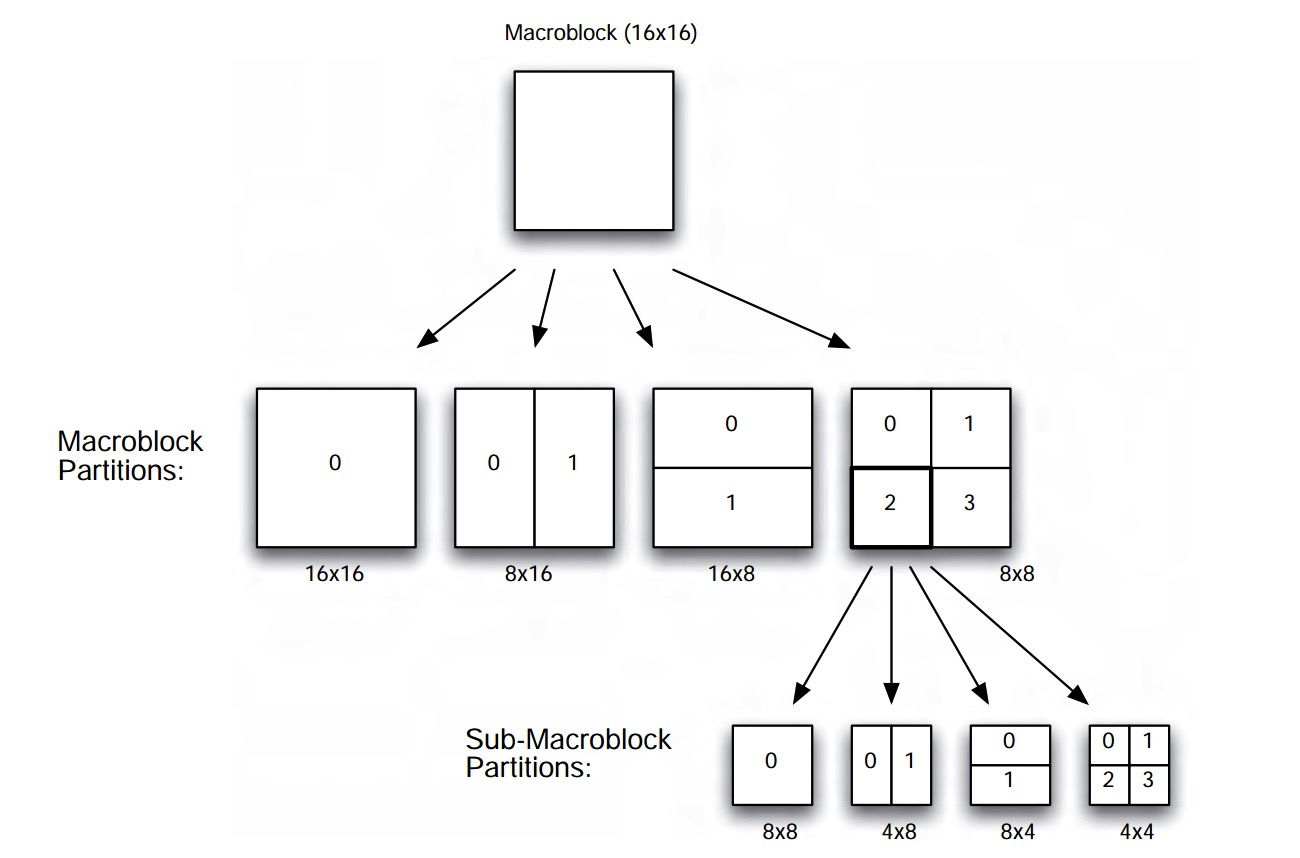
\includegraphics[height=8cm]{marcoblockpartition.jpg}
   \end{tabular}
   \end{center}
   \caption[mbpart] 
%>>>> use \label inside caption to get Fig. number with \ref{}
   { \label{fig:mbpart} 
Macroblock partitions and sub-macroblock partitions \cite{richardson2004h} }
   \end{figure}     % 在reference中引用
   
Each macroblock partition and sub-macroblock partition has one or two motion vectors (x, y). Each of them points to an area of the same size in a reference frame that is used to predict the current partition. Motion vectors for neighboring partitions are often highly correlated and so each motion vector is predicted from vectors of nearby, previously coded partitions. Motion vector is supposed to compensate the decoded picture from the reference ones. It means we could transmit the motion vector instead of the whole redundant of reference marcoblock.

\end{document}